
%Copyright (C) 2016 by Krishneel@JSK Lab, The University of Tokyo

%Copyright (C) 2016 by Krishneel@JSK Lab, The University of Tokyo

\documentclass{standalone}
\usepackage{footnote}
\usepackage{hyperref}
\usepackage{graphicx}
\usepackage{fancyhdr}

\renewcommand\footnoterule{%
  \kern-3\p@
  \hrule\@width2.5cm
  \kern2.6\p@
}
\makeatother

\begin{document}

\subsection{Platforms}
We customized the DJI developer platform M100 as shown in Fig.\ref{figure:task1-platform} (top). We used two Nvidia Jeston TX1 to distribute the heave computation load required for image processing. The two processors are connected via a wired internal network.
We also employed a camera with fisheye lens that has a $250^\circ$ wide viewing angle for tracking, as well as optical-flow $\&$ sonar sensor units to estimate the ego-motion of the UAV. The system framework is shown in Fig.\ref{figure:task1-platform} (bottom). The processing nodes inside the processors will be explained below.

\begin{figure}[h]
    \begin{center}
        \begin{minipage}{\hsize}
          \begin{center}
      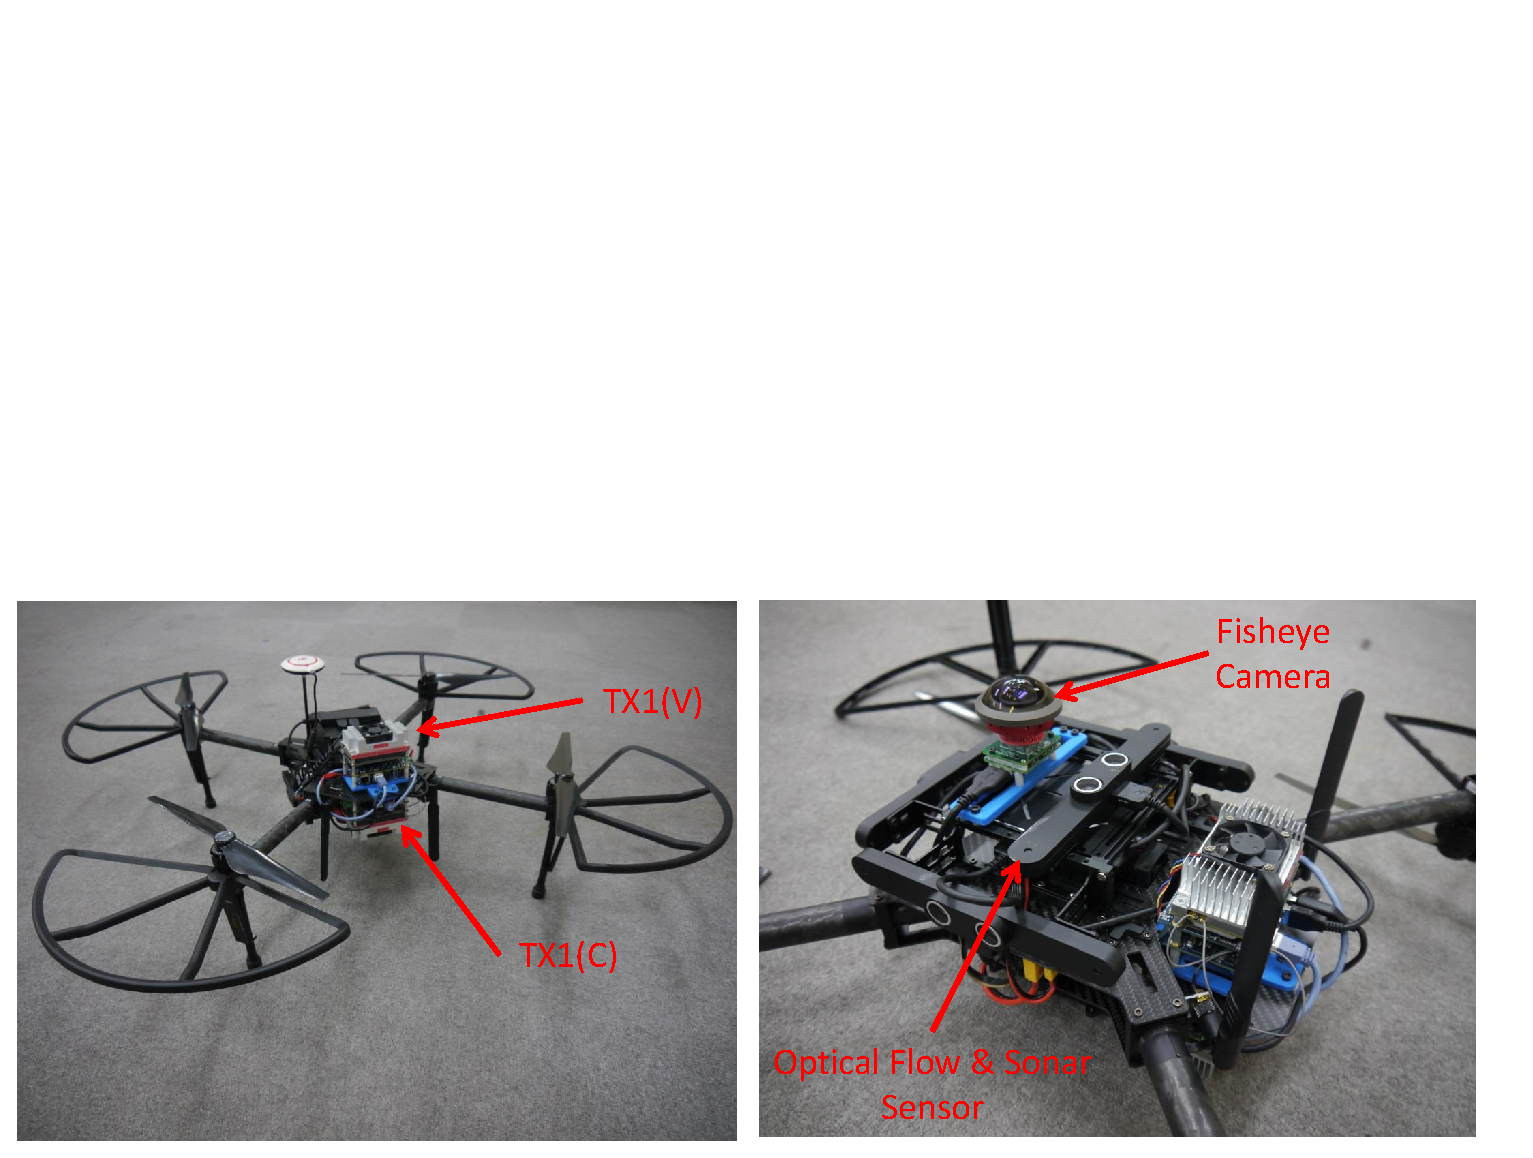
\includegraphics[clip, bb= 0 0 700 260, width=\columnwidth]{sections/task1/images/task1_hardware.eps}
          \end{center}
        \end{minipage}
        \begin{minipage}{1.0\hsize}
          \begin{center}
      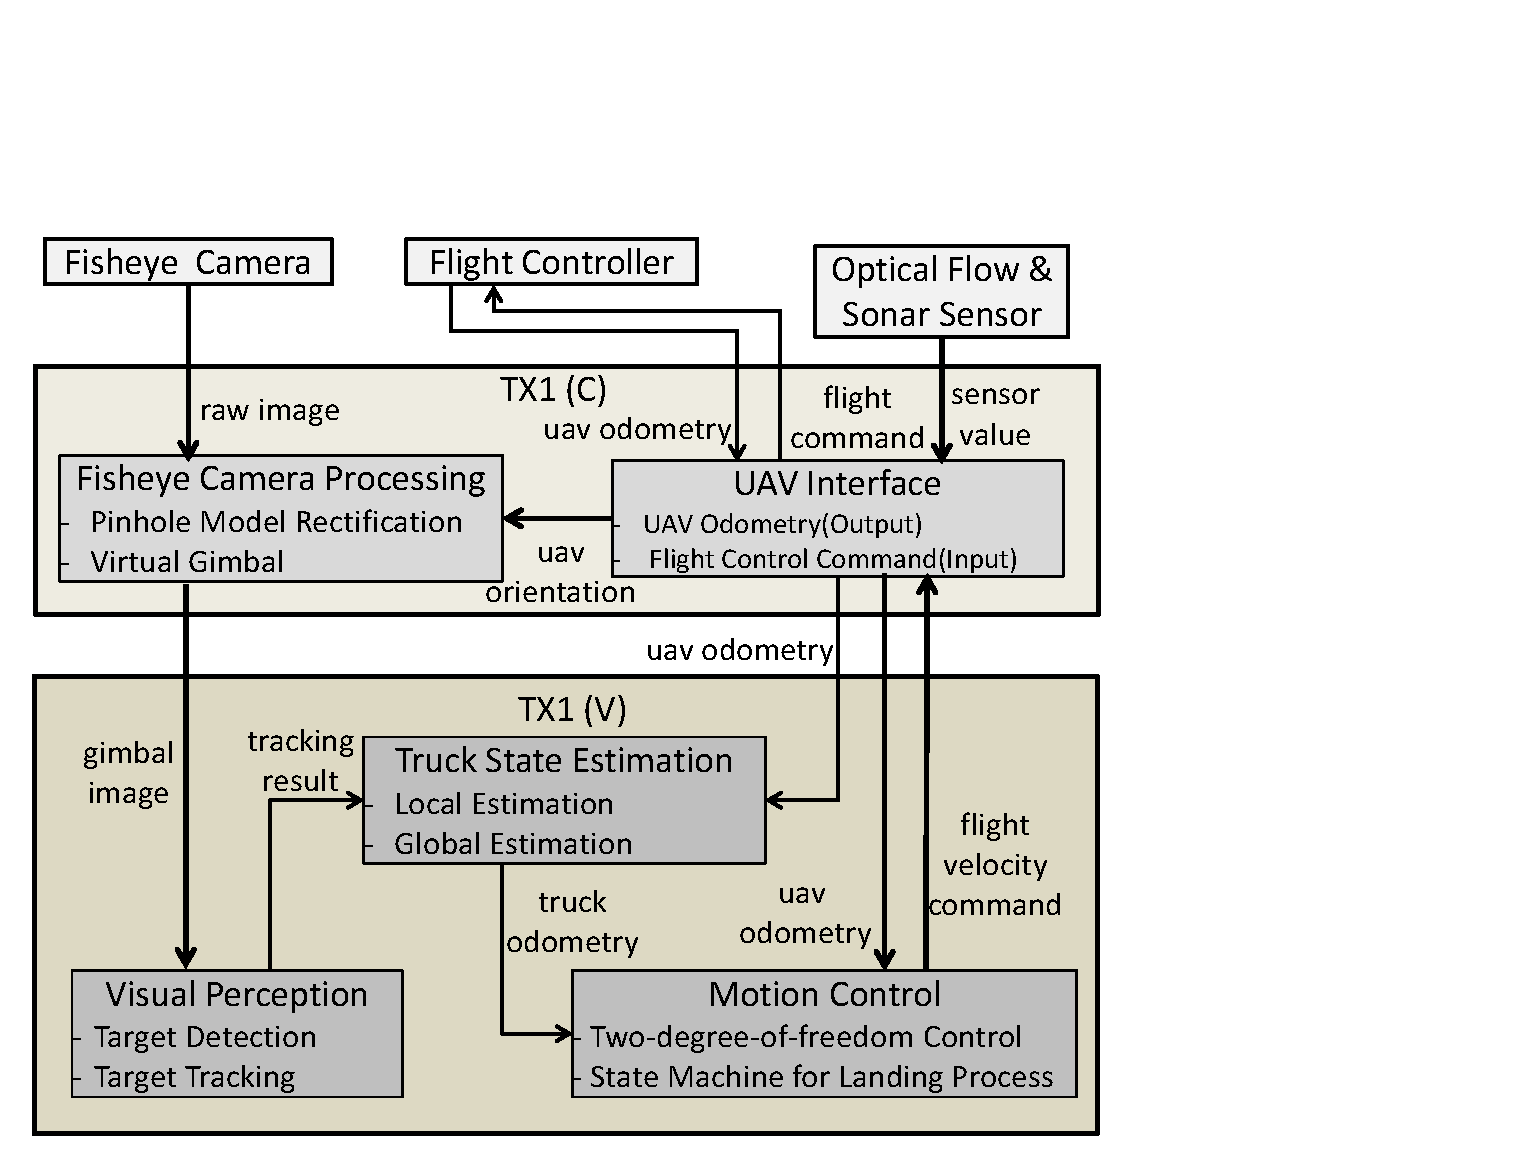
\includegraphics[clip, bb= 0 0 525 440, width=0.9\columnwidth]{sections/task1/images/task1_framework.eps}
          \end{center}
        \end{minipage}
    \end{center}
    \caption{Top: hardware platform DJI M100. Bottom: system diagram of the platform.}
    \label{figure:task1-platform}
\end{figure}


\subsection{Software Environment}
The visual perception algorithms and motion control are implemented
on Robot Operating System (ROS) environment\footnote{\url{http://www.ros.org}}.
We used Gazebo\footnote{\url{gazebosim.org}} for virtual simulations
\footnote{\url{https://github.com/start-jsk/jsk_mbzirc}}. Our
algorithms are implemented in C/C++, Python and CUDA-C.


\subsection{Visual Perception}

Image processing is one of the fundamental component of autonomous
systems. With efficient and robust image processing, planning and
decision making can be done more readily which improves the accuracy
and robustness of the execution of the assigned task. Hence, one of our
primary objective while designing our software architectures was
real-time performance with minimal loss of accuracy in image processing. The visual
component of task 1 includes three main stages described as follows:

\subsubsection{Fisheye Camera Processing}
To perform image processing using the images obtained from the fisheye camera, we first convert the raw images into pinhole model images. Furthermore, we also developed an original method called virtual gimbal, which combines the orientation data of UAV with the raw image data to calculate a stabilized image frame (Fig.\ref{figure:fisheye-virtual-gimbal}). This method is crucial when the UAV tilts with a large angle (e.g. greater than $20^\circ$) while tracking the downward target.

\begin{figure}[h]
    \begin{center}
      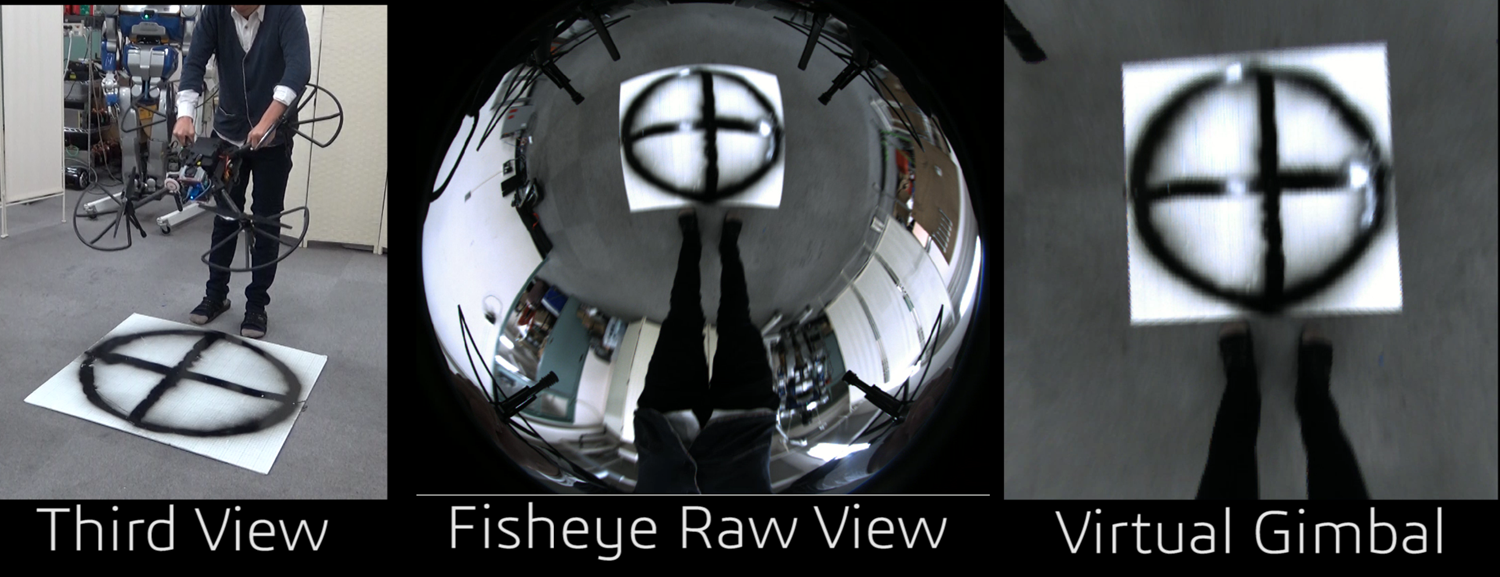
\includegraphics[width=0.9\columnwidth]{sections/task1/images/fisheye_virtual_gimbal.png}
    \end{center}
    \caption{Fisheye Virtual Gimbal}
    \label{figure:fisheye-virtual-gimbal}
\end{figure}

\subsubsection{Target Detection}
The target detection phase is the initial localization of the landing
region (heliport) on the truck. To detect the heliport we use a
traditional computer vision detection approach where by a sliding
window based method is used. However such raster scanning windows are
computationally expensive even for high end systems. To overcome this
crucial limitation we first generate candidate object
regions. Since the heliport is fixed to a moving target, we use
Gaussian based background subtraction fused with Kalman Filters for 
global motion compensation to generate regions of interest
(ROI)  with stable changes. The candidate ROI's are then ranked using
edge similarity between each sliding window. High scoring ROI are then
used for detecting the heliport using a pre-trained detector. 
In the following, let $\mathbf{H}$ denote the detected target region.

\subsubsection{Target Tracking}

In order for an UAV to approach and land on the heliport, online visual
feedback is very important since the target is constantly moving.
Using the assumption that the target is not
expected to change abruptly both in terms of visual motion and
appearances, we use visual tracking for online feedback.
The detected region $\mathbf{H}$ is used to initialize the
tracker. Our visual tracking algorithm is highly efficient and robust
to both scale and visual changes and runs in real time. Thus, it provides frame by frame location of the target. To enable a tracker
to run online in real time, we carefully crafted the expensive process
of feature computation by reducing it to a one time process. 
The invariant features for tracking are computed by passing the image
through several pre-trained kernels of varying dimensions. By varying
the sizes of the kernel, an approximate scale can also be detected.
Furthermore, the tracker is updated online at fixed intervals.

\begin{figure}[t!]
  \centering
  \includegraphics[height=1in]{sections/task1/images/detect2}
  \includegraphics[height=1in]{sections/task1/images/detect1}
  \caption{Illustration of truck and heliport detection.}
\end{figure}

\subsection{Truck State Estimation}

We can obtain the relative pixel position of a target object in the fisheye camera's image with the help of our visual perception algorithm. Furthermore, the UAV's state , including flying height, velocities, and rotation angles, can be obtained from sensors on the UAV. Using these information, the speed of target object in world coordinate can be calculated. Finally, with a low-pass filter's help, we can obtain a fairly accurate estimation of target velocity.

\subsection{Motion Control}

\subsubsection{Two-degree-of-freedom Control}

We present a two-degree-of-freedom control method including both feedforward and feedback method for truck tracking. Using the approach described in the previous section, a good estimation of the truck velocity can be obtained and used by a feedforward algorithm. Then, a PI controller can be used to make gentle adjustments to help the UAV maintain a position above the truck.

\subsubsection{State Machine for Landing Process}

We carefully designed a state machine for the landing process. We defined an inverted conical region relative to the center of the tracking object. When UAV is stably moving in this region, UAV is considered to be tightly keeping track of the moving object, and the UAV is allowed descend with a stable speed. Our strategy is that once the UAV is within 0.35[m] above the truck, we will stop its gradual descend and adjust the UAV's position to the center of the heliport and land directly and quickly to it. The reason is that currently our visual tracker detects the inside circle region of the heliport, whose radius is 0.5[m], and the fisheye camera we use has a $120^\circ$ viewing angle. This means that when the UAV is less than 0.29[m] above the heliport, the camera would not be able to see the whole heliport. 0.29[m] is a close enough distance for the UAV to land directly, and our experiments also proved that this strategy is feasible and practical.


\subsection{Results Achieved to Date}

We have completed the entire task one autonomously, landing on the 
target moving at 5[km/h], 10[km/h], and 15[km/h]. Moreover, we have demonstrated the effectiveness of our real time planning and tracking by showing the results of long duration
following of the target at over 35[km/h]. The results of these tracking and landing motion are shown in the progress video.

For landing control, we first tested our method to land on a static truck, and result shows that precision is within 10 centimeters, which is close to the results of a state-of-the-art work by HKUST's team who presented in ICRA2015. For a moving target, we succeeded in landing on the truck moving at 15[km/h] as shown in Fig.\ref{figure:landing}.

\begin{figure}[h]
    \begin{center}
      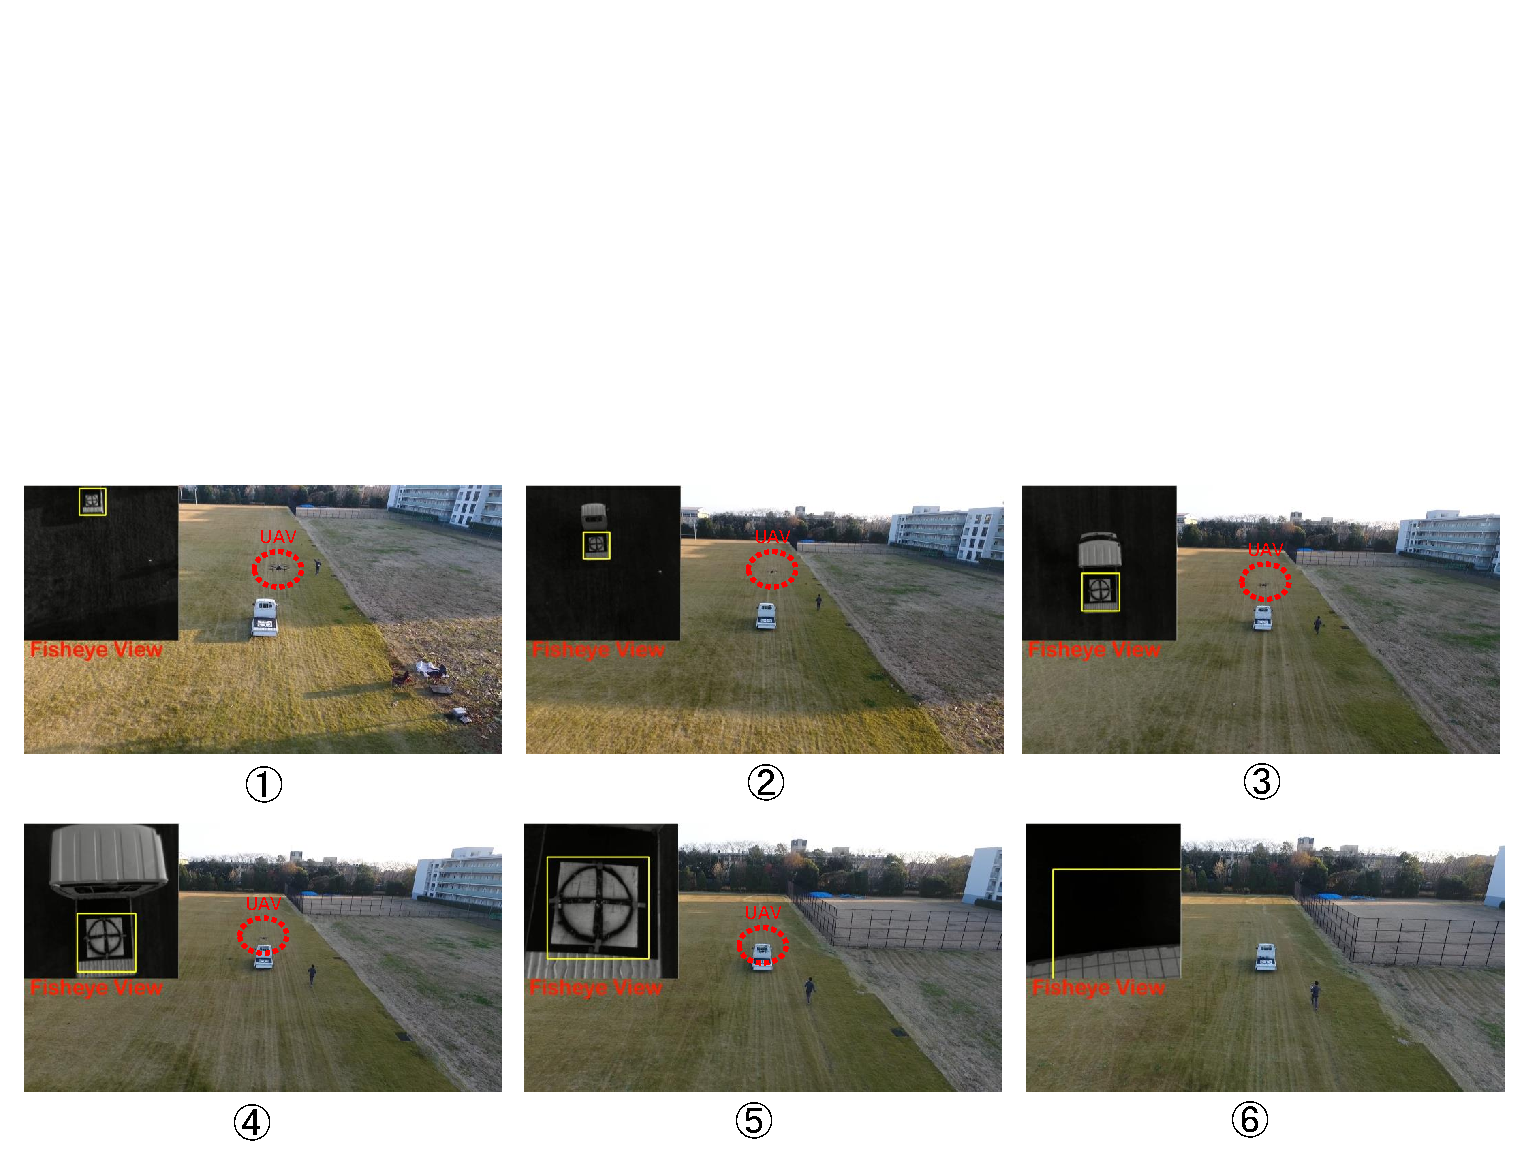
\includegraphics[clip, bb= 0 0 720 315, width=1.0\columnwidth]{sections/task1/images/task1_landing.eps}
    \end{center}
    \caption{The landing process in the case of [15km/h]. For more details, please see our video.}
    \label{figure:landing}
\end{figure}


\subsection{Future Work}
\subsubsection{Vision Algorithm}
Few improvements are required to increase the robustness of our
vision algorithms. First, we will add tracker drift recovery mode to
the visual tracking algorithm. Drift recovery will enable the
tracker to recover from drifting effects that may result from
occluded or lost target. Second, with the implementation of drift
recovery, we want the tracker to constantly update instead of updating at fixed
intervals. Such updating scheme will enable the tracker to adapt to
online visual changes without a need of prior learning.


\subsubsection{Landing Control}
Since outdoor landing when the target object is turning at a high speed is an unsolved difficult problem, currently our landing is also restricted in straight-road landing. However in the challenge, starting from the center crossroad, only a 20[m] straight road is available. Considering that the truck is moving at 15[km/h] (4.2[m/s]), the UAV has to land within 5[s]. Currently for development and safety consideration, our landing is slow and needs around 15[s].
In the next stage, we plan to re-evaluate these academic problems and make pioneer trails to generate realtime landing trajectories for landing then the target object is turning at a high speed.


\end{document}
